\documentclass[output=paper]{langsci/langscibook}
\author{Sonia Cyrino\affiliation{University of Campinas}}
\title{Brazilian Portuguese null objects and Spanish differential object marking}

% \chapterDOI{} %will be filled in at production

\abstract{Animacy features have been known to trigger syntactic phenomena. In
    this paper, I focus on \gls{DOM}, and the null object\is{null objects} in
    \glsdesc{BP}, where such features are relevant. I assume that \isi{animacy}
    corresponds to a specification of Person features, and lack of
    \isi{animacy} implies that no Person features are encoded in a DP\@.
    Furthermore, I propose that \isi{animacy} is encoded in a dedicated
    functional head\is{functional items}. Animate DPs (i.e.\
    DOM\is{differential object marking} in \ili{Spanish} and animate objects in
    BP) move to Spec, FP\tss{animacy}, a projection above V, below \emph{v}, to
    check a person\is{person features} feature. Crucially, inanimate DPs stay
    in situ. They are not DOM marked in \ili{Spanish} and, by virtue of being
low, they can be licensed as DP \isi{ellipsis} in BP\@.  This analysis may
contribute to work seeking to grasp the role of referential hierarchies in
syntax.}

\maketitle

\begin{document}\glsresetall

\section{Introduction}

The relevance of certain ``semantic/relational/accessibility hierarchies'' to
explain a number of syntactic phenomena in several languages has been
frequently noticed in the literature (\citealt{Silverstein1976,Aissen2003}
among others). In this view, nominal phrases should be ordered in accordance with
``referential/accessibility'' hierarchies (cf.\ \citealt{Aissen2003}).

In this paper, following ideas in \citet{Carnie2005} and \citet{Merchant2006},
I propose a syntactic approach to account for the role of \isi{animacy}
features.  Under my account, \isi{animacy} features trigger \isi{movement} of
the animate object to a position outside VP.

The paper is organized as follows: in \Cref{sec:key:27.2}, I present the
syntactic phenomena under scrutiny, that is, \isi{null objects} in Brazilian
Portuguese and \isi{differential object marking} in \ili{Spanish}. In
\Cref{sec:key:27.3}, I present my proposal, and in \Cref{sec:key:27.4}, I
review proposals in the literature and discuss how referential hierarchies can
be thought of in syntax.  The conclusion is that this analysis may contribute
to work seeking to grasp the role of \isi{animacy} features in syntax.

\section{Animacy and syntactic phenomena}\label{sec:key:27.2}

There are several different syntactic phenomena where the \isi{animacy} of the
nominal expressions seems to be crucially relevant. In this section, I focus on
null objects in Brazilian Portuguese and on \isi{differential object marking} in
Spanish. These are two phenomena that have been shown to be sensitive to
animacy features of the object DP in these languages.

\subsection{Null objects in Brazilian Portuguese}\label{sec:key:27.2.1}

Brazilian Portuguese (hereafter, BP) allows \isi{null objects} with specific
properties that differentiate them from the various types of \isi{null objects}
allowed in other languages \citep{CyrinoLopes2016}. It has long been noted
(\citealt{Omena1978,Pereira1981,Duarte1986}, among others) that
the antecedent of the null object\is{null objects} is [$-$animate], as in (\ref{ex:key:27.1}a) vs.\
(\ref{ex:key:27.1}b). However, a full pronoun is usually needed when the
antecedent is an inanimate DP with a specific reading (\ref{ex:key:27.2}a), or
when it is animate (\ref{ex:key:27.2}b):

\ea\label{ex:key:27.1}Brazilian Portuguese\\
    \ea
        \gll    A    estudante levou    o     livro   para  a     biblioteca
        depois   que  ela    leu~\textbf{$\varnothing$}.\\
                the   student      took     the   book  to       the   library after     that  she    read {}\\
        \glt    `The student took the book to the library after she read (it).'
    \ex
        \gll \llap{*}A  estudante  levou     o     menino   para   o cinema depois  que ela   beijou \textbf{$\varnothing$}.\\
                the   student       took     the  boy         to       the cinema after     that   she   kissed\\
        \glt
    \z
\z

\ea\label{ex:key:27.2}Brazilian Portuguese\\
    \ea
        \gll A    estudante levou    um   livro   para  a     biblioteca depois que  ela    leu \textbf{(ele)}\\
            the   student      took     a     book   to       the   library after     that  she  read \hphantom{(}it\\
        \glt `The student took a (specific) book to the library after she read (it).'
    \ex
        \gll A  estudante  levou  um menino para  o     cinema     depois  que ela    beijou \textbf{ele}.\\
                the student     took   a     boy       to       the cinema after that   she  kissed  him\\
        \glt    `The student took a (specific) boy to the cinema after she kissed him.'
    \z
\z
Besides this sensitivity to \isi{animacy},\footnote{There is sensitivity to
specificity as well, as seen in examples
(\ref{ex:key:27.1})--(\ref{ex:key:27.2}). I will come back to this issue in
\Cref{sec:key:27.3}.} anaphoric \isi{null objects} in BP, such as
(\ref{ex:key:27.1}a) have a cluster of properties that set them apart from the
\isi{null objects} of other languages (see \citealt{CyrinoLopes2016}).  First,
they may occur in \isi{islands} for \isi{movement}, unlike in \ili{European
Portuguese} \citep{Raposo1986} or Chinese \citep{Huang1984}. Additionally, they
do not allow their antecedents to be the subject of the matrix sentence, unlike
in \ili{Japanese} \citep{Ohara2007}. Finally, they allow strict and sloppy
readings, a property related to the possibility of \isi{ellipsis}
(\citealt{FiengoMay1984}, among others): sentence (\ref{ex:key:27.3}) is ambiguous: in
the strict reading Pedro's friend left Pedro's car in the street; in the sloppy
reading, however, Pedro's friend left his (own) car in the street:\footnote{BP
    is a language that allows \emph{v}P (V-stranding) \isi{ellipsis}, in which
    case the verb is the same in both clauses (i) (see
    \citealt{CyrinoMatos2005} for a distinction between \emph{v}P
    \isi{ellipsis} and \isi{null objects} in Portuguese):

\begin{exe}
    \exi{(i)}
    \gll Pedro escondeu seu dinheiro no armário, e    sua mãe   também escondeu \_\_\_.\\
        Pedro hid his money  in.the  closet    and  his  mother too  hid\\
    \glt \enquote*{Pedro hid his money in the closet and his mother did too.}
\end{exe}

In order to exclude the possibility for a \emph{v}P \isi{ellipsis} analysis of this
sentence, a different verb (\emph{guardou} `put/kept', \emph{deixou} `left') is
used in each clause in (\ref{ex:key:27.3}), and a PP is present to show that
only the object, and not the whole \emph{v}P, is elided.}

\ea\label{ex:key:27.3} Brazilian Portuguese\\
    \gll    Pedro guardou um carro na garagem, mas seu amigo deixou \textbf{$\varnothing$} na rua.\\
            Pedro put a     car       in.the   garage      but  his friend left {} in.the   street\\
    \glt    `Pedro put a car in the garage, but his friend left (it) in the street.'
\z
Because of these properties, \isi{null objects} have been analyzed as DP
\isi{ellipsis} by \citet{Cyrino1994,Cyrino1997}, that is, as inaudible DPs that
have identical antecedents.  This analysis is based on the fact that
\gls{BP}\il{Brazilian Portuguese} lost third person\is{person features}
clitics; in other words, these anaphoric elements were replaced by
\isi{ellipsis} due to a diachronic process relating the increase of certain
kinds of \isi{ellipsis} (see below) and the loss of third person\is{person
features} (inanimate) \isi{clitics}.

 European Portuguese, a language to which \gls{BP}\il{Brazilian Portuguese} is diachronically related, has
 always allowed the construction seen in (\ref{ex:key:27.4}), which was dubbed as
 ``propositional ellipsis'' by \citet{Cyrino1994,Cyrino1997}. In this
 construction, the elided sequence may be replaced by a neuter clitic
 \emph{o} `it', as in (\ref{ex:key:27.5}).  Interestingly (\ref{ex:key:27.4}), as
 opposed to (\ref{ex:key:27.5}), is grammatical in contemporary \gls{BP}\il{Brazilian Portuguese}:

\ea \label{ex:key:27.4} ✔ European Portuguese, ✔ Brazilian Portuguese\\
    \gll    Pedro vai casar amanhã   mas Maria  não sabe \textbf{$\varnothing$}.\\
            Pedro go marry tomorrow but   Maria  not  know\\
    \glt    `Pedro is going to get married tomorrow but Mary doesn't know (that Pedro is going to marry tomorrow / it).'
\z

\ea \label{ex:key:27.5} ✔ European Portuguese, ✘ Brazilian Portuguese\\
    \gll   Pedro vai    casar amanhã    mas Maria  não o sabe.\\
            Pedro go   marry tomorrow but Maria    not  it know\\
    \glt    `Pedro is going to get married tomorrow but Mary doesn't       know it.'
\z
Given these facts, \citet{Cyrino1994,Cyrino1997} argues that in European
Portuguese there has always been a free choice between the use of propositional
ellipsis or the neuter clitic \emph{o} in its place. The author shows that,
indeed, there are no changes through time in these constructions in the
European Portuguese diachronic data she investigated.

In contrast to European Portuguese, however, the \gls{BP}\il{Brazilian Portuguese} diachronic data
investigated by Cyrino show an important change in the occurrence of these
constructions. She found there is an increase for the \isi{ellipsis} option, and a
decrease in the use of the neuter clitic, as seen in \Cref{fig:key:27.1}.

\begin{figure}[htpb]
    \centering
    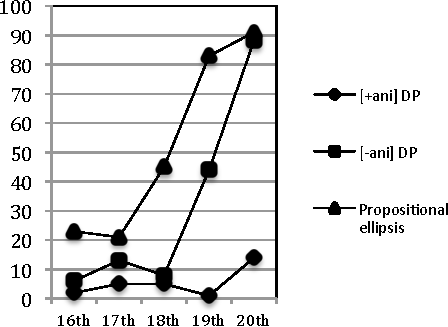
\includegraphics[width=.75\linewidth]{./img/fig27-1.pdf}
    \caption{Diachronic change for DP \isi{ellipsis} (null objects) and propositional
    \isi{ellipsis} (adapted from~\citealt{Cyrino1994,Cyrino1997})}
    \label{fig:key:27.1}
\end{figure}

\citet{Cyrino1994,Cyrino1997} proposes that there was an extension of the
ellipsis construction to other inanimate objects; therefore, the null object\is{null objects} in
BP has appeared with a property that is characteristic of \isi{ellipsis}, namely, the
strict/sloppy ambiguity seen above.

With respect to \isi{ellipsis}, it has been argued in the literature it must be
licensed by a functional head\is{functional items}
(\citealt{Lobeck1995,Kester1996}). In English, for example, \emph{v}P
\isi{ellipsis} is licensed by T, which has to be filled either with certain
auxiliaries or lexical \emph{be/have} \citep{Lobeck1995}. This allows an elided
\emph{v}P sequence to be possible.  Portuguese has V-raising, therefore, not
only auxiliaries, but also lexical verbs license \emph{v}P \isi{ellipsis},
since they move up to T \parencite{Matos1992,CyrinoMatos2002}. This kind of
\emph{v}P \isi{ellipsis} has been called V-stranding \isi{ellipsis}
(\citealt{Santos2009}, \citealt{Goldberg2005}) since the (auxiliary, lexical) V
is stranded in T and the remaining \emph{v}P is elided.

BP, however, has lost verb \isi{movement} to a high functional projection (T)
\citep{Galves2001}, and \emph{v}P \isi{ellipsis} is licensed by V in an Aspectual
head (\citealt{CyrinoMatos2002,CyrinoMatos2005};
\citealt{Cyrino2010,Cyrino2013}), that I assume in this paper is AspectOuter
(\citealt{MacDonald2008}).

As a consequence, both \emph{v}P \isi{ellipsis} and DP \isi{ellipsis} (null objects) can be
licensed, since they are c-commanded by V in a functional projection (lower
than T), contrary to what happens in European Portuguese (see
\citealt{CyrinoMatos2016}):

\ea\label{ex:key:27.6} Brazilian Portuguese \emph{v}P Ellipsis\\
    \ea
        \gll Ela tem lido   o   livro   para   as  crianças e ele     tem também   lido \textbf{$\varnothing$}.\\
            She has read   the   book to     the children and he   has   too read {}\\
        \glt `She has read the book to the children and he has too.'
    \ex {}[ \dots{} o livro para as crianças \dots{} ] \dots{} ele
    [\tss{T} tem] [\tss{VP\Aux} \tuple{tem}
    [\tss{Ad\emph{v}P} [\tss{Adv} também]
    [\textbf{\tss{Asp PerfP} }\textbf{lido}
    [\emph{\tss{\emph{v}}}\tss{P} \sout{o livro para as crianças} ]]]
    \z
\z
\citet{Cyrino2016}, based on \citet{CyrinoMatos2005}, proposes that the same
licensing mechanism is available for the null object\is{null objects} in BP\@.
The difference with \emph{v}P \isi{ellipsis} is that DP \isi{ellipsis} of the
object is licensed by the V in a lower aspectual head located between \emph{v}P
and VP, AspectInner (\citealt{MacDonald2008}; but see
\citealt{Lopes2014,Lopes2015}, for a more recent proposal on ``low ellipses''
for the null object\is{null objects} in BP):

\ea\label{ex:key:27.7} Brazilian Portuguese null object\\
    \ea
        \gll Ela tem lido o   livro para as   crianças  e ele tem também lido para as mães.\\
            She has read the book to  the children   and  he  has too read        to     the mothers\\
        \glt   `She has read the book to the children and he has also read it to   the mothers.'
    \ex \ob[ \dots{} o livro para as crianças \dots{} ] \dots{}  ele [\tss{T}
    tem] [\tss{VP\Aux} \tuple{tem} [\tss{Ad\emph{v}P}   [\tss{Adv}
    também] [\textbf{\tss{Asp PerfP}} lido [\tss{\emph{v}P} [\tss{AspInn}
    [AspInn+V \tuple{\textbf{lido}} [\tss{VP}   \tuple{V} [\tss{DP} o livro] para as mães]]]
    \z
\z
However, as shown by \textcite{Cyrino1994,Cyrino1997}, \gls{BP}\il{Brazilian
Portuguese} animate \isi{null objects} are possible in certain contexts:

\noindent\textbf{(a)} a \emph{v}P \isi{ellipsis} (V-stranding ellipsis) structure, where the whole
\emph{v}P is elided:

\ea\label{ex:key:27.8} Brazilian Portuguese\\
    \gll Lina disse  que   a   Maria beijou   o Pedro\tss{i} na         festa, e o   Paulo também disse que ela  beijou \textbf{$\varnothing$}.\\
         Lina said    that the Maria kissed   the   Pedro   at-the   party and the Paulo too       said   that  she kissed\\
    \glt    `Lina said that Maria kissed Pedro at the party, and Paulo said that she also did it.'
\z

\noindent\textbf{(b)} The antecedent is a bare plural or a non-specific
indefinite:

\ea\label{ex:key:27.9} Brazilian Portuguese\\
    \gll    Os tiras  insultavam [ presos / uns presos ]\tss{i} e depois   prendiam \underline{\hphantom{eles}}\tss{i} / *eles\tss{i}\\
            the cops   insulted {} prisoners {} some prisoners {} and afterwards {locked up} {} {} \hphantom{*}them\\
    \glt    `The cops insulted prisoners/some prisoners and afterwards locked (them) up.'
\z
These animate \isi{null objects} only occur in these specific structures, whereas the
inanimate null object\is{null objects} has no such restrictions.

Assuming that inanimate \isi{null objects} in \gls{BP}\il{Brazilian Portuguese} are
ellipsis, however, cannot be the full story since we have to explain why their
antecedents are [$-$animate], as seen in
(\ref{ex:key:27.1}) and (\ref{ex:key:27.2}). I come back to this issue in
\Cref{sec:key:27.3}.

\subsection{Differential object marking}\label{sec:key:27.2.2}

Certain accusative objects are marked (either morphologically or by a
preposition) in some languages when the object is [$+$animate] (and/or specific
in some cases, see below). This phenomenon has been called differential object
marking (hereafter, DOM).

Spanish is such a language: DOM\is{differential object marking} is manifested in the use of the preposition
\emph{a} `to' (which also marks datives) before animate objects:

\ea\label{ex:key:27.10} Spanish\\
    \ea
        \gll He     visto \textbf{*(a)} \textbf{tu} \textbf{padre}.\\
        have  seen   \hphantom{\textbf{*(}}to   your   father\\
        \glt `I saw your father.'
    \ex
        \gll He     visto \textbf{(*a)} \textbf{tu} \textbf{coche}.\\
            have  seen     \hphantom{\textbf{*(}}to  your car\\
        \glt `I saw your car.'
    \z
\z
Although specificity/definiteness (\citealt{Leonetti2004,Lopez2012}, among
others) has
been said to be involved in DOM\is{differential object marking}, \isi{animacy}
is still the most relevant feature for this phenomenon since, as pointed out by
\citet{Rodriguez-Mondonedo2007}, all animate indefinites (along with personal
pronouns and proper names) require DOM\is{differential object marking},
(\ref{ex:key:27.11}) and (\ref{ex:key:27.12}) (see
\citealt{Rodriguez-Mondonedo2007}):

\ea\label{ex:key:27.11} Spanish\\
    \ea
        \gll Vi *(a) alguien en el parque.\\
        saw \hphantom{*(}to somebody in the park.\\
        \glt `I saw somebody in the park.'
    \ex
        \gll No vi *(a) nadie en el parque.\\
            No saw \hphantom{*(}to nobody in the park\\
        \glt `I saw nobody in the park.'
    \z
\z\newpage

\ea\label{ex:key:27.12} \ili{Spanish}
    \ea
        \gll Vi (*a) algo en el parque.\\
               saw \hphantom{*(}to something in the park\\
        \glt `I saw something in the park.'
    \ex
        \gll No vi (*a) nada en el parque\\
            No saw \hphantom{*(}to nothing in the park\\
        \glt `I saw nothing in the park.'
    \z
\z
Several recent studies have proposed that DOM\is{differential object marking}
is the result of DP \isi{movement} to a position outside \emph{v}P driven by Case
requirements (\citealt{Torrego1998,
Rodriguez-Mondonedo2007,Lopez2012,OrmazabalRomero2013,Zdrojewski2013,OrdonezRoca2017}).
The first three analyses have in common the fact that they associate
\gls{DOM}\is{differential object marking} to a special configuration. However, each
one presents a different proposal for that configuration, as seen
below:\glsunset{DO}\glsunset{IO}

\ea\label{ex:key:27.13} \citet{Torrego1998}\\
    {}[\tss{\emph{v}P} DOM\is{differential object marking} [\tss{\emph{v}}
    \gls{EA} [\tss{\emph{v}}  \emph{v}   [\tss{VP}  V  \sout{DOM} ]]]]
\z

\ea\label{ex:key:27.14} \citet{Rodriguez-Mondonedo2007}\\ {}[\tss{DatP}
\emph{a}-\gls{DO} [\tss{Dat}  \Dat{} [\tss{\emph{v}P} \sout{\gls{DO}}
[\tss{\emph{v}} \emph{v} [\tss{VP} V \sout{\gls{DO}} ]]]]]
\z

\ea\label{ex:key:27.15} \citet{Lopez2012}\\
{}[\tss{\emph{v}P} \gls{EA} [\tss{\emph{v}} \emph{v} [\tss{αP}
(\emph{a})-\gls{DO} [\tss{α} \gls{IO} [\tss{α} α [\tss{VP} V \sout{\gls{DO}} ]]]]]]
\z
The structures in (\ref{ex:key:27.4})--(\ref{ex:key:27.6}) show some
differences: (i) in the projection to which the marked direct object moves, and
(ii) on the nature of that projection.\footnote{As for the nature of the
    projection to which the DOM\is{differential object marking} object moves
    to, the proposals also differ. For Torrego, \emph{a} is itself a head that
    has nominal properties.  \citeauthor{Rodriguez-Mondonedo2007} claims
    \emph{a} is not present in syntax and it simply reflects Case at a
    morphophonological level.  López assumes that \emph{a} is in a head K that
selects for the direct object, and Spell Out rules will dictate whether the
head is pronounced or not.  In other words, for López \emph{a} is one of the
possible options for the pronunciation of the head K that dominates the DP\@.}
For \citet{Torrego1998}, the DOM\is{differential object marking} object sits in
the second specifier of a \emph{v}P projection that introduces the \gls{EA}.
\textcite{Rodriguez-Mondonedo2007} does not refer explicitly to specific
position for the external argument, but \textcite{Lopez2012} argues that
DOM\is{differential object marking} objects are lower than external arguments,
and they move to a dedicated head between \emph{v}P and VP\@. This, according
to him, explains the contrast one finds in (\ref{ex:key:27.16}), where the
DOM\is{differential object marking} object does not c-command the external
argument.\newline

\ea\label{ex:key:27.16} \ili{Spanish}
    \ea[*]{%
        \gll Ayer       no   atacó       su\tss{i} propio padre   a ningún\tss{i} niño.\\
            yesterday  not   attacked    his own    father   to   no child\\
        \glt intended: `Yesterday no father attacked his own child.'}
    \ex[]{%
        \gll Ayer       no   atacó         ningún\tss{i} padre   a   su\tss{i} propio   niño.\\
          yesterday  not   attacked      no          father   to  his    own child\\
        \glt `Yesterday, no father attacked his own child.'}
    \z
\z
López assumes that postverbal subjects in \ili{Spanish} stay \emph{in situ}. In
(\ref{ex:key:27.16}a), the possessive pronoun cannot have a bound reading,
triggered by the negative DP inside the direct object. In (\ref{ex:key:27.16}b),
the external argument c-commands the DOM\is{differential object marking} object and, therefore, the bound
reading is possible.

In what follows, I briefly review the proposals that make reference to the role
of \isi{animacy} and specificity.

\citet{Rodriguez-Mondonedo2007} assumes that \emph{a} is the spell out of
Dative Case and has Person features. Crucially, he assumes \emph{v}P is the
projection of a head that only has Number features and because of the lack of
Person, it cannot check Case. Therefore, personal pronouns, definite and
animate DPs and indefinite human DPs move to spec \emph{v}P, but since they
cannot check Case because \emph{v} lacks [Person] features, they have to move
up to the specifier of DativeP, where Case can be checked because of the
presence of relevant Number and Person features -- that is where they get the
mark \emph{a}. Non-DOM objects (non-specific inanimate DPs) get Accusative Case
in the specifier of \emph{v}P because they crucially only have Number features
and do not have Person features. Their (Number) features\is{number features}
can be checked in Spec\emph{v}P.

\textcite{Lopez2012}, however, proposes an αP projection that seems to
integrate Rod\-rí\-guez-Mondoñedo's DatP and the aspectual head proposed by
\citet{Torrego1998}. He suggests that this projection is used to define the
aspectual structure of the verb. Besides that, he proposes that direct objects
come in two classes: simple DPs and complex DPs. The latter are selected by a
head K: they will be a KP structure and will be marked by \emph{a}: [\tss{KP} a
[\tss{DP} ]]. These two classes of objects have different semantic
interpretations. Unmarked objects are predicates, \tuple{e,t} type, and undergo
incorporation with the verb. The effect is a restriction of the verbal
predicate followed by \emph{Existential Closure}:

\ea\label{ex:key:27.17}
    [\tss{VP} [\tss{V} comer] [\tss{D/N/NumP} patatas]]
\z
However, the head K is a semantic function that takes an object of the type
\tuple{e,t} and produces \tuple{e}, an individual. Therefore, KP, which is not \tuple{e,t},
cannot occur as the complement of a verb. The unmarked object \tuple{e,t} can
incorporate to satisfy its Case, whereas KP, in order to get Case, is merged
with SpecαP, a position which is selected by \emph{v}P:

\ea\label{ex:key:27.18}
    {}[\tss{\emph{v}P}  v [\tss{αP}  KP [\tss{α}  α  VP ]]]
\z
It is interesting to notice that, in López's proposal, both animate and
inanimate objects could be in SpecαP, but not all of them would be
\emph{a}{}-marked. In his proposal the position is not responsible for the
\emph{a}{}-marking. For López, \emph{a}{}-marking occurs as a consequence
of Spell Out rules that make reference to the KP context (properties of the DP,
the NP, and the thematic and aspectual properties of the verb). He proposes
that there is no direct mapping between syntax and semantics, but a pairing
between syntactic positions and different modes of semantics composition.
Specificity effects are the by-product of both the scrambling of the direct
object to a position above its base position and the semantic operation of
\emph{choice function.} For López αP is, thus, a projection
identified with a cluster of aspectual and applicative properties and it will
be the correct context for K (in KP) to be realized as \emph{a} provided that
other conditions including \isi{animacy} are also satisfied.

\citet{OrmazabalRomero2013} investigate DOM\is{differential object marking} and
its relation with object \isi{clitics} in some varieties of \ili{Spanish}. They assume that
object agreement\is{agreement!object agreement} and Case assignment are linked and that there is only one
position available for their morphological expression. They propose a structure
as \eqref{ex:key:27.19}:

\ea\label{ex:key:27.19}
    {}[\tss{\emph{v}P} [\tss{DP} \emph{a} los niños]  [\tss{\emph{v}} \gls{EA}
    [\tss{\emph{v}} \emph{v} [\tss{VP}  V  [\tss{DP} \sout{los niños} ]]]]]
\z
A [$+$animate] DP must be licensed by agreement. Therefore, it must move to
Spec, \emph{v}P. \emph{A-}marking is the result of this checking relation.
Indefinite and [$-$animate] DPs are not \emph{a-}marked because they
incorporate. Crucially, the authors assume that the dative\is{dative case} clitic \emph{le} is
object agreement\is{agreement!object agreement} marking in \emph{v}. Therefore, when there is an
\emph{a-}marked object (\emph{a} is an agreement marking), the
DOM\is{differential object marking} object competes with the dative\is{dative case} clitic for
the same position. This explains the contrast in
(\ref{ex:key:27.20}):

\ea\label{ex:key:27.20} \ili{Spanish}
    \ea[*]{%
        \gll    Le enviaron   a   todos   los       heridos         a la     doctora.\\
                \Cl{}  sent.\Pl{}    to  all.\Pl{} the.\Pl{}  wounded.\Pl{} to  the  doctor\\}
    \ex[]{%
        \gll    Le   enviaron todos   los       heridos         a   la doctora.\\
               \Cl{}  sent.\Pl{}    all.\Pl{}   the.\Pl{} wounded.\Pl{} to  the  doctor\\
        \glt `They sent all the wounded to the doctor.'}
    \z
\z
\textcite{OrdonezRoca2017} also assume DOM\is{differential object marking}
involves an extra functional projection that is responsible for a checking
relation necessary for certain objects. They assume \citegen{Kayne2005}
proposal of prepositions as probes, and they consider \emph{a} is a preposition
that is inserted in the derivation:

\ea\label{ex:key:27.21}
    [\tss{\emph{v}P} [\tss{v$'$} [ \emph{v} \tn{v}{[accusative]}  [\tss{αP} KP
    \tn{kp}{[uCase]} [\tss{α$'$} α [\tss{VP} V \sout{KP} ]]]]]
    \ta{v.south}{kp}{Agree}\vspace{2em}
\z
The crucial assumption for Ordoñez \& Roca is that, contrary to \ili{English},
Spanish \emph{v} does not license [$+$animate, +specific] DPs; consequently
DOM\is{differential object marking} objects cannot stay in situ: \ili{Spanish}
has an extra mechanism for object licensing: the preposition \emph{a} is
crucially present in the numeration.  Additionally, the derivation has the same
steps as causatives in \ili{French}; in other words, all transitive
constructions in \ili{Spanish} bearing an animate or specific object such as
(\ref{ex:key:27.22}) will have the operations in (\ref{ex:key:27.23}):

\ea\label{ex:key:27.22}
    Vimos a Maria
\z

\ea\label{ex:key:27.23}
    \ea \dots{}  [\tss{\emph{v}P}  \emph{v}  [\tss{VP} vimos   [\tss{DP} María ] ] ]    DP [$+$anim, +spec]
    \ex Merge of \emph{a}\\
        \dots{}  a  [\tss{\emph{v}P}  \emph{v}  [\tss{VP} vimos   [\tss{DP} María ] ] ]
    \ex Movement to Spec\\
    \dots{}  [\tss{\emph{a}P} [María]\tss{i}  a  [\tss{\emph{v}P}
        \emph{v}  [\tss{VP} vimos [t]\tss{i} ] ] ]
    \ex Merge of W\\
        \dots{}  W [\tss{\emph{a}P} [María]\tss{i}  α  [\tss{\emph{v}P}
        \emph{v}  [\tss{VP} vimos [t]\tss{i} ] ] ]
    \ex Head raising\\
        \dots{}  [\emph{a}\tss{j}+W] [\tss{\emph{a}P} [María]\tss{i}  t\tss{j}
        [\tss{\emph{v}P}  \emph{v}  [\tss{VP} vimos [t]\tss{i} ] ] ]
    \ex Remnant movement\\
        \dots{}  [\tss{WP}  [\tss{\emph{v}P}  \emph{v}  [\tss{VP} vimos
        [t]\tss{i} ]]]\tss{k} [\emph{a}\tss{j}+W] [\tss{\emph{a}P} [María]\tss{i}  t\tss{j}  t\tss{k}
    \z
\z
In sum, different authors assume different positions with respect to the
specific Case \emph{a} is encoding, Dative or Accusative. All of them,
however, assume that the DOM\is{differential object marking} object is in a higher position than the unmarked
object. In other words, it seems that there is a consensus in that inanimate
DPs remain in situ.\largerpage[-1]

\subsection{Are null objects in \gls{BP} instances of DOM?}\label{sec:key:27.2.3}

Interestingly, as seen above, sensitivity to \isi{animacy} (and specificity) is a
well-known characteristic of DOM\@. A natural question is then: can overt vs.\
null objects in \gls{BP}\il{Brazilian Portuguese} be an effect of differentially marking the object in the
language? Indeed, there have been previous accounts relating \gls{BP}\il{Brazilian Portuguese} to \ili{Spanish}
DOM\@.

Within a functionalist framework, \citet{SchwenterSilva2002} and
\citet{Schwenter2006} have claimed that the null object/full pronoun pattern
found in \gls{BP}\il{Brazilian Portuguese} is reminiscent of DOM\is{differential object marking} in \ili{Spanish}.  They notice that full pronouns
in \gls{BP}\il{Brazilian Portuguese} might be comparable to DOM\is{differential object marking} objects in \ili{Spanish} since both are likely to be
[$+$animate, $+$specific] while also receiving morphological marking
(\emph{a} in \ili{Spanish}, full pronoun in BP). On the other hand, as seen above,
anaphoric \isi{null objects} in \gls{BP}\il{Brazilian Portuguese} are likely to be [$-$animate, $-$specific], just
like the bare objects (i.e.\ those without \emph{a}) in \ili{Spanish}.

Yet, there might appear to be a problem with this understanding of DOM\is{differential object marking} and
\gls{BP}\il{Brazilian Portuguese} overt vs.\ \isi{null objects}. If the latter
correspond to the unmarked form, it is unclear why they may have the ``Spanish
DOM requirement'' of being \emph{specific}\footnote{This does not automatically
    imply that DOM\is{differential object marking} objects in \ili{Spanish} must always be [$+$specific]. The problem
    seems to arise from the tendency (in many descriptive, and also more formal
    accounts) to obligatorily connect DOM\is{differential object marking} with
    \enquote{specificity}. However, as
    discussed in the more recent literature, there are certain syntactic
    contexts where objects which cannot be understood in terms of specificity
    are nevertheless DOM\is{differential object marking} marked (e.g., negative quantifiers, clause union
configurations, etc.). What seems to unite DOM\is{differential object marking}
is rather a \emph{syntactic configuration} \parencite{Lopez2012}, and not
necessarily descriptions in terms of \enquote{specificity}.}  (even in the
absence of \isi{animacy}).\footnote{But recall, from \eqref{ex:key:27.9}, that
    non-specific animate \isi{null objects} are possible in
    \gls{BP}\il{Brazilian Portuguese}, and as also shown by
    \textcite{Cyrino1994,Cyrino1997}. I will come back to these cases in
\Cref{sec:key:27.3}.}\largerpage[-2]

This observation however does not invalidate the connection with DOM\@. It
rather shows that, within \ili{Romance}, \gls{BP}\il{Brazilian Portuguese} is
more similar to languages like \ili{Romanian} than \ili{Spanish} in that,
descriptively, two conditions must be simultaneously met for differential
marking: [$+$animate] and [$+$specific]
(\citealt{Farkas1985,Dobrovie-Sorin1994,IrimiaCyrino2015}, among others). The
presence of only one of these \enquote{features} is not normally enough to
trigger DOM\is{differential object marking} in \ili{Romanian}, while it might
do so in \ili{Spanish} more frequently. For example, as shown by
\citet{IrimiaCyrino2015,IrimiaCyrino2017}, in \ili{Romanian} animates do not
obligatorily have differential marking; animates can be used without
DOM\is{differential object marking}, if interpreted non-specific, as shown in
(\ref{ex:key:27.24}a), just like \isi{null objects} in BP\@. In \ili{Spanish}
animates, as seen above, require DOM\is{differential object marking} in
non-intensional contexts, regardless of specificity (see
also~\citealt{Lopez2012,Leonetti2008}, among others), as can be seen in
(\ref{ex:key:27.25}):\footnote{Also, inanimates do not easily accept
    differential marking in \ili{Romanian}, even if interpreted specifically,
    demonstrating that specificity is not what triggers DOM\@. Clause-union
    contexts of the type in (i) generally require DOM\is{differential object
    marking} in \ili{Spanish} (see \citealt{Lopez2012}, among others):

\begin{exe}
    \exi{(i)} Romanian\\
        \gll Au văzut \textbf{(*pe)} nişte avioane căzând.\\
            \Aux.\Tpl.\Prs.\Indic{} seen \hphantom{(*}\textsc{dom} some planes fall.\Ger{}\\
        \glt `They saw planes falling from the sky.'
\end{exe}}

\ea\label{ex:key:27.24} Romanian\\
    \ea
        \gll Ion         a                                 văzut un         om.\\
             John        \Aux.\Tsg{}.\Prs{}.\Indic{}      seen a.\M.\Sg{}    man\\
        \glt `John saw a man.'
    \ex
        \gll Ion       l-a văzut pe un om.\\
        John     \Cl.\Tsg.\M-\Aux.\Tsg{}.\Prs.\Indic{} seen \textsc{dom} a.\M.\Sg{} man\\
        \glt `John saw a specific man.'
    \z
\z

\ea\label{ex:key:27.25} Spanish\\
    \gll Juan    vió \textbf{*(a)} un hombre.\\
        John    see.\Pst.\Tsg{}  \hphantom{\textbf{*(}}\textsc{dom} a.\M.\Sg{}    man\\
    \glt `John saw a man.'
\z
If \isi{null objects} in \gls{BP}\il{Brazilian Portuguese} are DP \isi{ellipsis} licensed
by the lexical V in AspInn, and unrestricted \isi{null objects} are only possible
when the antecedent is [$-$animate], the impossibility of restricted null
objects has to be linked to the fact that DP \isi{ellipsis} is not licensed. The
question is thus: why are animate objects not licensed under ellipsis? The
answer must reside in the syntactic composition strategies available for
categories like \enquote{animacy}. In other words, if animate objects move to a
higher position (as in DOM\is{differential object marking}) they cannot be
elided since they will not be licensed by V in AspInn.

\section{Animacy in syntax}\label{sec:key:27.3}

The discussion above shows that \isi{animacy} is relevant for syntactic phenomena in
BP and \ili{Spanish}. In this section, I advance a proposal to account for null
objects in \gls{BP}\il{Brazilian Portuguese} and its relation to DOM\@.

In a nutshell, I propose, following \citet{Richards2008}, that [$\pm$Person]
features are inherent to different nominals. Animacy in syntax can be
implemented as the result of the \isi{movement} of a [$+$Person] or [$-$Person] DP to
the specifier of functional category (call it F\tss{[Person]}) that has an
uninterpretable ([\emph{u}Person]), probably to value Case (see also Ordoñez
\& Roca forthcoming). DPs that are [$-$animate] (i.e.\ those that are
Person-less) and non-specific do not move out of \emph{v}P, since they are
φ-incomplete, and they value Case in-situ (by the φ-incomplete probe \emph{v},
as in \citealt{Rodriguez-Mondonedo2007}).

\citet[140]{Richards2008} proposes that Person is an exclusive (syntactic)
property of (definite) and animate nominals: a person\is{person features}
specification on indefinites and inanimates is redundant, since these DPs will
always be third person\is{person features}, and thus would plausibly be left
unspecified, as seen in~\tabref{tab:key:27.27.1}.

\begin{table}
\begin{tabularx}{\textwidth}{XXXXX}
\lsptoprule
& \multicolumn{2}{c}{Person--animacy} & \multicolumn{2}{c}{Person--definiteness}\\
   & Animate & Inanimate & Definite & Indefinite\\
\midrule
1  & ✔       & ✘         & ✔        & ✘\\
2  & ✔       & ✘         & ✔        & ✘\\
3  & ✔       & ✔         & ✔        & ✔\\
\lspbottomrule
\end{tabularx}
\caption{Reverberations of the \enquote{Person} feature in syntax (adapted from
\citealt{Richards2008})}\label{tab:key:27.27.1}
\end{table}

According to Richards, indefinites and inanimates will bear only number (and
gender) features D; they are thus \enquote{defective} in the agreement system
(in the sense of \citealt{Chomsky2001}). Given that Bare Nouns are always
inherently third-person, Richards assumes that Person is a property of the
category D, not N. Bare Plurals lack D, so they are \enquote{Person-less}.
First and second person\is{person features} pronouns will always be DPs,
whereas third person\is{person features} nominals may be either DPs or NPs,
depending on whether their Person feature is syntactically specified or not
(e.g.\ bare plurals are NPs in his proposal). He assumes that ``if indefinites
and inanimates lack Person (as claimed above), then this equates syntactically
to their lacking a DP structure -- that is, they are bare NPs''
\citep[140]{Richards2008}.

Therefore, \isi{animacy} in syntax is the result of [$\pm$Person] feature
checking.\footnote{In Richard's system, as can be seen in \tabref{tab:key:27.27.1},
definites also have a Person feature. Although definiteness, specificity has
been related to \isi{null objects} in \gls{BP}\il{Brazilian Portuguese} and DOM\is{differential object marking} in \ili{Spanish}, the role of Person in
the construction of definiteness will not be examined in detail in this paper.
See below the discussion on this issue.} Richards examines \enquote{prominence
scales} proposed in the functionalist literature and translates their effects
into feature checking. In his account, the presence or absence of features as
Person provide a syntactic basis for various phenomena: (i) a Person
specification implies an animate interpretation at the interface; for example,
agreement restrictions in the \isi{Person Case Constraint} phenomenon; (ii) a
Person-less probe may assign (value) a different Case from its nondefective
[$+$Person] counterpart in the Probe--Goal-Agree system of \citealt{Chomsky2001}
(this would be the case of DOM); (iii) the \gls{EPP}\is{Extended Projection Principle}-feature of a probe may be
associated with the entire probe (i.e. Person + Number) or else with just the
Person feature of the probe, yielding differential argument movements (Object
Shift would be a case in point).  The author assumed that, besides unvalued
features, there is an \gls{EPP}\is{Extended Projection Principle} feature on the probe. This is to justify that
\emph{v} only probes for Person.\is{PCC|see{Person Case Constraint}}

I concentrate on the fact that [Person] is a relevant feature for \isi{animacy} (and
leave definiteness and specificity for now, but see \citealt{IrimiaCyrino2015},
in progress, and below). Thus, I assume \isi{animacy} as related to the need of
checking [$\pm$Person] in syntax. Differently from Richards, I assume that Bare
Plurals are defective and lack person\is{person features} in D,  and inanimate DPs have a
\enquote{Person-less} D. In other words, [$\pm$Person] is encoded in D, but lack of
Person features does not entail lack of D, since D will still have other
features as Number, Gender.\footnote{Number is actually encoded in D in
\gls{BP}\il{Brazilian Portuguese}, even in a null D, see
\citet{CyrinoEspinal2015}.}

\tabref{tab:key:27.2} summarizes my proposal:\footnote{A reviewer asks why
    third person animates are treated as [$-$Person], since it would be equally
    feasible to have first/second person\is{person features} as
    [$+$participant, +person], and animate third person\is{person features} as
    [$+$person].  I think the problem with that is that there would be a
    redundancy for first and second person\is{person features}, since
    participants are necessarily [$+$person]. In my system it is clearer that
    the third person\is{person features} is the \enquote{non-person}, as son
many times it has been suggested in the linguistic literature.}

\begin{table}
\begin{tabularx}{\textwidth}{XX}
\lsptoprule
First/Second person\is{person features} & [$+$Person]\\
Third person\is{person features} animate & [$-$Person]  \\
Third person\is{person features} inanimate/ Bare Plurals & \enquote{Person-less} \\
\lspbottomrule
\end{tabularx}
\caption{Animacy and Person features \citep{Cyrino2016}}\label{tab:key:27.2}
\end{table}

Transitive \emph{v}s in \gls{BP}\il{Brazilian Portuguese}, as in \ili{Spanish}
\parencite{Rodriguez-Mondonedo2007,OrdonezRoca2017}, do not have [Person]
features, and they are φ-incomplete.  Case is only valued for matching DPs,
\emph{v}s are not able to value Case in animate DPs, because the latter are
φ-complete.  Therefore, they have to move to value Case.

A functional head\is{functional items} (call it F\tss{[Person]}) located below
\emph{v}P and above AspInn is able to value Case to those DPs that match that
feature.  Therefore, the effects of \isi{animacy} in syntax comes from the
\isi{movement} of a [$+$Person] or a [$-$Person] DP to the specifier of a
functional category that has [Person].

In sum, [$-$animate] (i.e.\ Person-less) DPs do not move out of \emph{v}P, they are
φ-incomplete, and have Case valued by the φ-incomplete probe
\emph{v} (as in \citealt{Rodriguez-Mondonedo2007}). On the other hand,
[$+$animate] (i.e.\ [$+$Person] or [$-$Person]) DPs are φ-complete, so they move
to the specifier of F\tss{[Person]} to value Case.

The behavior of \gls{BP}\il{Brazilian Portuguese} null vs.\ overt objects seen in \eqref{ex:key:27.26} can be understood as
the possibility for AspInn to license \isi{ellipsis}, something only possible for
inanimate objects since they stay in situ, as seen in the structure in
\eqref{ex:key:27.27}:

\ea\label{ex:key:27.26} Brazilian Portuguese\\
    \ea[]{%
        \gll O estudante levou   o   livro     para  a     biblioteca depois que {leu \textbf{$\varnothing$}}.\\
            The student   took     the   book   to       the   library after that read \\
        \glt `Pedro took the book to the library after he read (it).'}
    \ex[*]{%
        \gll O estudante  levou  o    menino   para  casa    depois que   o professor expulsou \textbf{$\varnothing$}.\\
          the student     took   the boy       to       house   after   that the teacher      expelled\\}
    \z
\z

\ea\label{ex:key:27.27}
    \emph{v} [\tss{AspInnP} [\tn{asp}{\tss{V+Asp}} leu [\tss{VP}  \tuple{V} \tn{goal}{\sout{o livro}} ]]]
    \ta{asp.south}{goal}{ellipsis licensing}\vspace{2em}
\z
In \ili{Spanish}, these DPs are not DOM-marked, as shown by
\textcite{Rodriguez-Mondonedo2007}.

Animate DPs, with some exceptions, cannot be null; the object has to be spelled
out as a full pronoun, exemplified by \emph{ele} in (\ref{ex:key:27.28}).
Animate DPs are [$-$Person]; therefore, they move out of \emph{v}P to Spec,
F\tss{[Person]} (= DOM\is{differential object marking} \isi{movement}){} and value Case.

\ea\label{ex:key:27.28} Brazilian Portuguese\\
    \gll O   estudante levou   o     menino para  casa     depois  que o professor  expulsou \textbf{ele}.\\
         the student     took   the  boy       to       house   after     that the teacher    expelled him\\
    \glt `The student took the boy home after the teacher expelled him.'
\z

\ea\label{ex:key:27.29}
    {}[ \emph{v} [\tss{F[Person]P} \textbf{ele\tss{[$-$Person]}}
    F\tss{[Person]}\tss{} [\tss{AspInnP} [\tss{V+AspInn} expulsou [ V \tuple{ele\tss{[$-$Person]}} ]]]
\z
Notice that a full pronoun, such as \emph{ele} in (\ref{ex:key:27.16}a) above
and \emph{ela} in (\ref{ex:key:27.30}) below, can also refer to a [$-$animate]
antecedent; this indicates there is a Person-less pronoun in \gls{BP}\il{Brazilian Portuguese} (like
\emph{it} in \ili{English}):

\ea\label{ex:key:27.30} Brazilian Portuguese\\
    \gll O     tira   puxou [a arma]\tss{i} e depois escondeu \underline{\hphantom{ela}}\tss{i} ela\tss{i}\\
          the  cop  drew    the   gun      and afterwards hid {} it\\
    \glt `The cop draw the gun and afterwards hid it.'
\z
Interestingly, the inanimate full pronoun has a distinct distribution from its
animate counterpart, as shown by \citet{Galves2001}:

\noindent\textbf{(a)} Inanimate full pronouns (\ref{ex:key:27.31}a) cannot occur
in a short answer as opposed to the animate ones (\ref{ex:key:27.31}b):

\ea\label{ex:key:27.31} Brazilian Portuguese\\
    \ea
        \gll Q:  O     que     você   deixou  em   casa?         A: *Ele.\\
        {}     The what   you     left    at      home {} \hphantom{*}It\\
        \glt \hphantom{Q: }`What did you leave at home?'
    \ex
        \gll Q:  Quem   você   deixou  em   casa?              A: Ele.\\
            {} Who     you     left       at     home          {} him\\
        \glt \hphantom{Q: }`Who did you leave at home?' -- `Him.'
    \z
\z

\noindent\textbf{(b)} Inanimate full pronouns (\ref{ex:key:27.32}a) cannot  occur
in contrastive focus, as opposed to the animate pronouns (\ref{ex:key:27.32}b):

\ea\label{ex:key:27.32} Brazilian Portuguese\\
    \ea[*]{%
        \gll Eu vi     ele   (e     não ela) (o     livro   e     não a     revista).\\
        I   saw  it-\M{} \hphantom{(}and   not   \hphantom{(}it-\glossF{}  the book and  not   the magazine\\
        \glt}
    \ex[]{%
        \gll Eu vi     ele (e     não   ela) (o     João e     não a Maria).\\
                I   saw him \hphantom{(}and   not   her    \hphantom{(}the   João and not the Maria\\
        \glt `I saw him (and not her) (João and not Maria).'}
    \z
\z
\textcite{IrimiaCyrino2015,IrimiaCyrino2017} show that there is a crucial
difference between overt pronouns in \gls{BP}\il{Brazilian Portuguese} in terms of their specificity features.
Comparing the overt pronouns in \gls{BP}\il{Brazilian Portuguese}, which are the correspondent of DOM-marked
objects in \ili{Romanian}, the authors show that, although \textcite{Lopez2012}, as
seen above, proposes DOM\is{differential object marking} objects are outside \emph{v}P but below \emph{v},
there must be other positions for DOM\@. Specific DOM-objects in \gls{BP}\il{Brazilian Portuguese} (i.e.\ the
animate/inanimate overt pronouns) and in \ili{Romanian} (\emph{pe}-marked DPs) must
be interpreted above \emph{v}P.\glsunset{DO}\glsunset{EA}

\ea\label{ex:key:27.33}
    \tss{} \dots{} \gls{DO}.\textbf{\textsc{dom}} [\tss{\emph{v}P} \gls{EA}
    [\tss{αP} \sout{\gls{DO}.\textbf{\textsc{dom}}} α [\tss{V} V \sout{\tuple{DO}} ]]]
\z
Irimia \& Cyrino base their observation on wide/narrow scope interpretation of
indefinite objects in the scope of modal adjectives. \ili{Romanian} \eqref{ex:key:27.34} and \gls{BP}\il{Brazilian Portuguese} \eqref{ex:key:27.35}
are alike in that ``DOM-marked'' objects (i.e.\ \emph{pe}{}-marked DPs in
Romanian and overt animate/inanimate pronouns in BP)  are interpreted as being
outside the quantificational domain of modal adjectives (i.e.\ outside
\emph{v}P), and thus they do not allow narrow scope:\footnote{Inanimate null
objects in \gls{BP}\il{Brazilian Portuguese}, however, allow both wide and narrow scope (ia), since they are
inside \emph{v}P; animate \isi{null objects} are possible only if non-specific, as shown by
the impossibility of wide scope (ib), which shows they do not move:

\begin{xlist}
    \exi{(i)}
        \ea
            \gll    Pedro considera um livro necessário (para o   projeto) e vai comprar \textbf{$\varnothing$}.\\
                    Pedro  considers a    book necessary for   the project  and go buy\\
            \glt    a book >> necessary; necessary >> a book
        \ex
            \gll    Pedro considera um estudante necessário (para o   projeto) e   vai contratar \textbf{$\varnothing$}.\\
                    Pedro considers  a    student necessary    for   the project  and go hire\\
            \glt    *a student >> necessary; necessary >> a student
        \z
\end{xlist}
This shows, as expected, that in order for the null object\is{null objects} to be licensed (as
DP \isi{ellipsis}, with V raising to AspInn), it must be inside VP, and null
objects allow wide scope for inanimate antecedents only.  This scenario is
expected as \gls{BP}\il{Brazilian Portuguese} (inanimate) indefinites appear to be quantificational like the
Romanian ones, and thus can get a specific interpretation in a quantificational
position above VP but below \emph{v}P as argued by
\citet{IrimiaCyrino2015,IrimiaCyrino2017}. Crucially, the nature and positions
of \enquote{specificity} readings with quantificational indefinites are
different than those of \enquote{specificity} with DOM\is{differential object
marking} (see also \citealt{Lopez2012} for conclusions in the same direction).
Thus, it appears that there are at least two \enquote{specificity} positions in
Romanian and \gls{BP}\il{Brazilian Portuguese} -- one inside \emph{v}P (but
above VP), which is quantificational and allows reconstruction in
\citeapos{Diesing1992} and \citeapos{May1985} terms, and another one, outside
\emph{v}P (which is argumental, can host differential marking, and does not
allow reconstruction) (see \citealt{IrimiaCyrino2015}, in progress).}

\ea\label{ex:key:27.34} Romanian\\
    \ea
        \gll Consideră \textbf{o}    \textbf{studentă} necesară       (pentru un proiect).\\
        consider     a   student.\glossF.\Sg{} necessary.\glossF.\Sg{}   \hphantom{(}for a project)\\
        \glt a student $>$ consider; consider $>$ a student
    \ex
        \gll (O)      consideră \textbf{pe} \textbf{o} \textbf{studentă} necesară.\\
        \hphantom{(}\Cl.\Tsg.\glossF.\Acc{} considers  \textsc{dom}  a student.\glossF.\Sg{}        necessary.\glossF.\Sg{}\\
        \glt a student $>$ consider; *consider $>$ a student
    \z
\z
\newpage
\ea\label{ex:key:27.35} Brazilian Portuguese\\
    \ea
        \gll Pedro considera um estudante necessário (para o projeto) e     vai contratar \textbf{ele}.\\
              Pedro considers a    student      necessary     \hphantom{(}for   the project and go   hire         him\\
        \glt a student $>$ necessary; *necessary $>$ a student
    \ex
        \gll Pedro  considera um   livro   necessário   (para o projeto) e vai   comprar \textbf{ele}.\\
            Pedro   considers a       book   necessary   \hphantom{(}for   the   project and go     buy         it\\
        \glt a book $>$ necessary; *necessary $>$ a book
    \z
\z
These facts show that, since specific indefinites with overt pronouns as well
as animates in \gls{BP}\il{Brazilian Portuguese} do not allow a narrow scope reading, they must be outside
\emph{v}P. Thus \gls{BP}\il{Brazilian Portuguese} is similar to \ili{Romanian}, but different from \ili{Spanish} with
respect to how specificity interacts with \isi{animacy} for DOM\@.

A final question I have to answer in this section is: what about Bare Plural
antecedents for \isi{null objects} in BP\@? As seen above, animate and
inanimate null objects are possible in \gls{BP}\il{Brazilian Portuguese} if the
antecedent is a bare plural ((36), (37)) and not when it is a full DP
(\ref{ex:key:27.36}b):

\ea\label{ex:key:27.36} Brazilian Portuguese\\
    \ea
        \gll Os   tiras    insultavam [ presos ]\tss{i} e depois prendiam \underline{\hphantom{eles}}\tss{i} / *eles\tss{i}\\
          the   cops   insulted {} prisoners {} and   afterwards {locked up} {} {} \hphantom{*}them\\
        \glt  `The cops insulted prisoners and afterwards locked (them) up.'
    \ex
        \gll Os   tiras   insultavam   [ os presos ]\tss{i} e depois prendiam *\underline{\hphantom{eles}}\tss{i} / eles\tss{i}\\
           the  cops  insulted {} the prisoners {} and afterwards {locked up} {} {} them\\
        \glt `The cops insulted the prisoners and afterwards locked them up.'
    \z
\z

\ea\label{ex:key:27.37} Brazilian Portuguese\\
    \gll Os   tiras    puxavam \ob{} armas \cb{}\tss{i} e depois escondiam \underline{\hphantom{elas}}\tss{i} / *elas\tss{i}\\
        the   cops   drew       {} guns {}       and   afterwards hid {} {} \hphantom{*}them\\
    \glt `The cops drew guns and afterwards hid (them).'
\z
Interestingly, notice that Bare Plurals are non-specific and, as seen in
\tabref{tab:key:27.2}, they are Personless. Therefore, they always stay in situ,
and \isi{null objects} are always allowed for those antecedents, as seen in the
structures in \eqref{ex:key:27.38}:

\ea\label{ex:key:27.38}
    \ea \emph{v} [\tss{AspInnP} [\tn{vasp}{\tss{V+Asp}} insultavam [\tss{VP}
    \tuple{V} \tn{goal}{\sout{presos}} ]]]
        \ta{vasp.south}{goal}{ellipsis licensing}\vspace{2em}
    \ex \emph{v} [\tss{AspInnP} [\tn{vasp}{\tss{V+Asp}} puxavam [\tss{VP}
    \tuple{V} \tn{goal}{\sout{armas}} ]]]
        \ta{vasp.south}{goal}{ellipsis licensing}\vspace{2em}
    \z
\z
Other possible animate \isi{null objects}, seen above in (\ref{ex:key:27.22}),
repeated here as (\ref{ex:key:27.39}a), are not really DP \isi{ellipsis}, since they
occur as the result of verbal (\enquote{V-stranding}) \isi{ellipsis}. In those cases,
the V in AspOuter licenses \emph{v}P \isi{ellipsis} in BP\@. See the simplified
structure in (\ref{ex:key:27.39}b) (see also
\citealt{Cyrino2013,ReintgesCyrino2016}):


\ea\label{ex:key:27.39} \ili{Brazilian Portuguese}
    \ea
        \gll    Lina disse  que   a   Maria beijou   o Pedro\tss{i} na festa, e o Paulo também disse que ela  beijou \textbf{$\varnothing$}.\\
                Lina said    that the Maria kissed   the   Pedro   at-the   party and  the Paulo too       said   that  she kissed\\
        \glt    `Lina said that Maria kissed Pedro at the party, and Paulo said that she also did it.'
    \ex
        {}[ \dots{} beijou o Pedro na festa \dots{} ] \dots{} ela [\tss{AdvP} [\tss{Adv} também] [\textbf{\tss{AspOuter}} \textbf{beijou} [\tss{\emph{v}P} \sout{o Pedro na festa} ]]]\\
    \z
\z
In sum, I have shown in this section that \emph{animacy}, considered as Person
features encoded in a functional projection and triggering \isi{movement}, is the key
factor to explain \isi{null objects} in \gls{BP}\il{Brazilian Portuguese} and
DOM\is{differential object marking} in \ili{Spanish}.

\section{On referential hierarchies and syntax}\label{sec:key:27.4}

Several linguistic phenomena have been related to hierarchies of grammatical
categories, specially in typological and functionalist studies (for example,
\citealt{Silverstein1976}, among others). These hierarchies make reference to
the referentiality of nominal expressions and to the likelihood of their
appearing with certain \isi{grammatical functions} or having certain markings. As
such the following is a common proposed hierarchy:

\ea\label{ex:key:27.40}
    pronouns1/2 $>$ pronouns 3$>$ humans $>$ animates $>$ inanimates \citep{Silverstein1976}
\z
This hierarchy is based on data from languages that have a split in their case
alignment system according to different nominal expressions. Thus, first and
second person pronouns appear higher in the hierarchy (being more to the left),
than third person\is{person features} pronouns. This corresponds to different
case marking: subjects that are higher receive nominative\is{nominative case}
whereas lower subjects receive \isi{ergative case}.

\textcite{Aissen1999,Aissen2003} proposes that such hierarchies can be treated
in the Optimality Theory framework (\glsunset{OT}\gls{OT}), placing the
well-known generalizations in grammatical theory. Her hierarchy
(\ref{ex:key:27.41}) aims to explain DOM\@. If a direct object that corresponds
to any nominal expression in the hierarchy can be DOM-marked in a language,
then the objects that are higher in the hierarchy can be so marked.

\ea\label{ex:key:27.41} Animacy and Definiteness Hierarchies \citep{Aissen2003}
    \ea Animacy Hierarchy\\
        Human $>$ Animate $>$ Inanimate
    \ex Definiteness Hierarchy\\
        personal pronoun $>$ proper name $>$      definite NP $>$ specific
        indefinite NP $>$ non-specific NP
    \z
\z
\citet{CyrinoDuarteKato2000}, analysing \isi{null subjects} and \isi{null objects}
in \gls{BP}\il{Brazilian Portuguese}, proposed a hierarchy that would be relevant for language acquisition\is{language acquisition}.
Thus, for a language that has the internal option of null categories, one of
the factors that may influence this choice is the \isi{animacy} status of the
antecedent. If a language has an empty category for a certain element, it will
also have empty categories for other elements that are lower in a ``referential
hierarchy'':

\ea\label{ex:key:27.42} Referential Hierarchy
    (\citealt{CyrinoDuarteKato2000})\\
    \begin{tabular}{@{}l@{ $>$ }l@{ $>$ }l@{ $>$ }l@{}}
    non-argument & proposition & [$-$human] & [$+$human]\\
    \multicolumn{4}{@{}l}{third p. $>$ second p. $>$ first p.}\\
    \multicolumn{4}{@{}l}{[$-$specific] $>$ [$+$specific]}\\
    \multicolumn{1}{@{}l@{}}{[$-$referential]} &
    \multicolumn{2}{@{}l@{}}{$\xleftarrow{\hspace{4.5em}}\hspace{-.25em}\xrightarrow{\hspace{4.75em}}$} & \multicolumn{1}{@{}l@{}}{[$+$referential]}\\
    \end{tabular}
\z
For example, for the null object\is{null objects} in \gls{BP}\il{Brazilian Portuguese}, if the input presents a pronoun or
clitic in a lower position in the hierarchy, the child, in the process of
language acquisition\is{language acquisition}, will consider it a weak pronoun that occurs in a head or
argument position. All the higher positions will be lexical pronouns. If the
input has a null object\is{null objects} for a referential antecedent, the child will assume
that all the lower positions in the hierarchy can be null.

However, hierarchies are not explanations -- they reveal effects that should be
better explained in a theory of grammar
\parencite[see][]{Carnie2005,Merchant2006,BrownKochWiltschko2004}. In this
line, the relevant features could be seen as effects of the position of nominal
expressions in the structure as a consequence of either the mapping between
syntactic structure and argument structure/semantics
\parencite{Diesing1992,Jelinek1993,Meinunger2000,JelinekCarnie2003,Carnie2005,Merchant2006,Platzack2008}
or certain syntactic operations \parencite{Richards2008,Barany2015,Cyrino2016}.
In this paper, I focused on the latter possibility.

In fact, as seen in this paper, inanimate objects have a different behavior
with respect to animate objects in several languages; the generalization
appears to be that they stay in situ. This suggests that we may consider the
referential hierarchies described above as the by-product of syntactic
structure.

Many instances of such generalization are present in the literature. There are
languages as Blackfoot (spoken in Alberta province in Canada) in which
transitivity and \isi{animacy} are marked on the verb by means of certain suffixes,
the \emph{verb class finals}. \citet[66]{Bliss2010}, following
\citet{RitterRosen2008}, \citet{Brittain2003}, \citet{Hirose2001} and
\citet{Mathieu2006}, proposes that these suffixes are manifestations of
\emph{v.}  Transitive animate suffixes introduce arguments in a higher
position than transitive inanimate ones, as seen in the structure in
(\ref{ex:key:27.43}):

\ea\label{ex:key:27.43}
    [\tss{\emph{v}P2} \textsc{anim} [\tss{\emph{v}$'$}  \Ta{} [\tss{\emph{v}P1}
    \textsc{anim}  [\tss{\emph{v}$'$} \textsc{ti} [\tss{VP}  [\tss{V} root] \textsc{inan}]]]]]\\
\z
In a sentence as (\ref{ex:key:27.44}), the verbal root \emph{a'pihk} shows up with
the intransitive inanimate suffix \emph{ahto} followed by the benefactive
transitive animate suffix \emph{-omo.}

\ea\label{ex:key:27.44} Blackfoot \citep[67]{Bliss2010}\\
    \gll    An-wa     Rosie nit-a'pihk-ahto-omo-ok-wa ot-inaka'simik.\\
        \Dem-\Prox{} Rosie 1-sell-\Ti-\Ben-\Inv-\Prox{} 3-car\\
    \glt    `Rosie sold me her car.'
\z
This is predicted if the underlying order is as in \eqref{ex:key:27.43}. After
V \isi{movement}, the resulting surface order will be V-\Ti-\Ta-(\Ben), as seen
in \eqref{ex:key:27.44}.

Moreover, in Sesotho,\il{Sotho} as shown by \textcite{DemuthMachobaneMoloiOdato2005},
there is a specific order for the occurrence of two internal arguments. If the
animacy feature of the two internal arguments (objects) are the same, any one
can appear immediately adjacent to the verb. However, if one is [$+$animate],
then it must immediately follow the verb, no matter its θ-role.

Object agreement\is{agreement!object agreement} is also related to \isi{animacy} in certain languages. In
\ili{KiRimi} \parencite{Hualde1989,Woolford2000}, dative\is{dative case} constructions show
Dative Alternation.  In the oblique option (the PP Dative), the animate direct
object agrees with the verb. However, in the Double Object
Construction,\is{double object construction}
agreement is blocked when the direct object is also animate, since the verb
agrees with the animate indirect object.

Likewise in \ili{Mohawk} \citep{Baker1996}, animate objects need to be licensed
either by incorporation to the verb or by agreement with the auxiliary\is{auxiliaries} verb.
Since incorporation with animates is very restricted, the preferred option is
agreement with animate objects. Inanimate objects, however, never trigger
agreement with the verb. In applicative constructions in this language, the
benefactive/goal argument must be licensed via agreement with the verb (it
never incorporates); the theme, if animate, loses its ability to agree with the
verb, since in this language only one of the objects shows agreement. When the
direct object is animate, then, the only possible agreement is with the
benefactive argument, that then incorporates even if it is animate.

Another instance of the relevance of \isi{animacy} features in syntax is the
case of \emph{leísmo} and the \gls{PCC}\is{Person Case Constraint}. The former
refers to an extension of the third person dative\is{dative case} clitic
\emph{le} to contexts where one would expect the accusative  \emph{lo}
(masculine form) or \emph{la} (feminine form).
\citet[319--320]{OrmazabalRomero2013} point out that in \emph{leísta} dialects
of \ili{Spanish}, \isi{clitics} are not marked for Case, but for \isi{animacy}.
Thus the third person direct object distinguishes \isi{animacy}: when it is
[$-$animate], these dialects use \emph{lo}/\emph{la} (\ref{ex:key:27.45}); when
it is animate, they use \emph{le}, the same form of the dative\is{dative case}
(\ref{ex:key:27.46}).

\ea\label{ex:key:27.45} \emph{Leísta} Spanish\\
    \gll    Lo vi.\\
            \Tsg{}.\textsc{do} vi\\
    \glt    `I saw it (the book).'
\z

\ea\label{ex:key:27.46} \emph{Leísta} Spanish\\
    \gll    Le vi.\\
            \Tsg{}.\textsc{do}   vi\\
    \glt    `I saw him/her (the boy/the girl).'
\z
Finally, the Person-Case Constraint is also subject to \isi{animacy} requirements, as
shown by \citet{OrmazabalRomero2007,OrmazabalRomero2013}. The authors propose that \isi{animacy} has
an important role: the clitic \emph{le} is, as seen above in \emph{leísta}
dialects, the mark for a [$+$animate] nominal. The \gls{PCC}\is{Person Case
Constraint} only occurs when \emph{le} is occurring:\newpage

\ea\label{ex:key:27.47} \ili{Spanish}
    \ea[*]{Te lo di.\\
        (\emph{te} = second person\is{person features} dative\is{dative case};
    \emph{lo} = third person\is{person features} accusative [$-$animate])}
    \ex[*]{Te le di.\\
        (\emph{te} = second person\is{person features} dative\is{dative case};
    \emph{le} = third person\is{person features} accusative [$+$animate])}
    \z
\z
This section shows that there are many other phenomena that are sensitive to
animacy features. This suggests they may be considered under the proposal
advanced in this paper, namely, that there is a functional projection
(furnished with Person features) which is responsible for checking and
triggering \isi{movement} of animate objects, thus resulting in their different
behavior with respect to inanimate ones. The further exploration of these
phenomena, however, lies outside the scope of this paper but is undergoing
current investigation.

\section{Conclusion}

With the proposal advanced in this paper, we may explain why the occurrence of
null objects in \gls{BP}\il{Brazilian Portuguese} is restricted to inanimate
DPs. In the same way, \isi{differential object marking} in \ili{Spanish} finds a suitable
analysis. As for the phenomena described in \Cref{sec:key:27.4}, a more
detailed analysis under this proposal is being conducted
\parencite{Cyrino2017}, since in all of them the idea that \isi{animacy} triggers
movement may provide a proper explanation for the difference in syntactic
effects. My proposal predicts, with some caveats, that if two internal
arguments occur, where one is animate and the other is inanimate, the former
will move out of its base position to a position higher than the latter.

Besides these results, we may also conclude that referential hierarchies
described in the functional literature can be mapped from syntactic structure.
Besides \isi{animacy}, specificity seems to also be at play in the phenomena
investigated in this paper. In \ili{Romance} it seems specificity is occupying
a higher projection (i.e.\ above F\tss{person}) triggering \isi{movement} (see
\citealt{IrimiaCyrino2015}) for interpretation purposes (see
\citealt{Lopez2012}), leading us to conjecture a syntactic hierarchy as:

\begin{center}
\begin{tabular}{lll}
    αP          & $>$ & F\tss{person}\\
    Specificity & $>$ & Animacy
\end{tabular}
\end{center}

Although more detailed exploration is necessary with respect to other features,
I see this contribution as a promising line of research.\newpage

\printchapterglossary{}

\section*{Acknowledgements}

I would like to acknowledge the support of the following grants: CNPq ---
\emph{Conselho Nacional de Desenvolvimento Científico e Tecnológico} (Grant
303742/2013-5), and FAPESP -- \emph{Fundação de Amparo à Pesquisa do Estado de
São Paulo} (Grants 2012/06078-9 and 2014/17477-7). Parts of this paper were
presented at the Department of Linguistics Colloquium Series at Stony Brook
University in February 2016, at the Workshop \emph{Uma viagem diacrônica 20
anos depois} held at the University of Campinas in June 2016, and at the
\emph{VIII Romania Nova Workshop} held at the University of Buenos Aires in
November 2016. I would like to thank the audiences in these conferences for
their feedback. I am also grateful to the reviewers for their careful reading,
invaluable comments and suggestions.  Shortcomings are my own responsibility.

{\sloppy
\printbibliography[heading=subbibliography,notkeyword=this]
}

\end{document}
